\documentclass{article}
\usepackage[utf8]{inputenc}
\usepackage[a4paper, top=1in, bottom=1in, left=1in, right=1in]{geometry} 
\usepackage{graphicx}
\setlength\parindent{0pt} % Removes all indentation from paragraphs - comment this line for an assignment with lots of text
\usepackage[]{algorithm2e}
\usepackage{amsmath}
\usepackage{amssymb}
\usepackage{tikz}
\usepackage{pgfplots}

\newcommand\tab[1][1cm]{\hspace*{#1}}
\newcommand{\vect}[1]{\boldsymbol{#1}}

\title{\textbf{Machine Learning Note}}
\author{Chauncey Liu}
\date{\today}

\begin{document}
 
\maketitle
 
\tableofcontents

\newpage
 
\section{Introduction}
\subsection{What is Machine Learning}
A computer program is said to learn from experience E with respect to some task T and some performance measure P, if its performance on T, as measured by P, improves with experience E.

\subsection{Supervised Learning}
Supervised learning is a type of machine learning algorithm that uses a known dataset (called the training dataset) to make predictions.\\

Supervised Learning: "Right" answers given \\
Regression: Predict continuous valued output \\
Classification: Disrete valued output \\

\begin{tabular}{|c|c|c|} 
  \hline
  Input(x) & Output(y) & Application \\
  \hline
  \hline
  Home feature & Price & Real Estate \\ 
  \hline
  Ad, user info & Click on ad? (0/1) & Online Advertising \\
  \hline
  Image & Object (1, ... , 1000) & Photo Tagging \\
  \hline
  Audio & Text transcript & Speech Recognition \\
  \hline
  English & Chinese & Machine Translation \\ 
  \hline
  Image, Radar info & Position of other cars & Autonomous driving \\
  \hline
\end{tabular}

\subsection{Unsupervised Learning}
Unsupervised learning is a type of machine learning algorithm used to draw inferences from datasets consisting of input data without labeled responses.\\

\section{Linear Regression with One Variable}
\subsection{Model and Cost Function}
\subsubsection{Model Representation}
How do we represent hypothesis h? Use methods like regression to generate a classifier.
\subsubsection{Cost Function}
Hypothesis: $h_\theta(x) = \theta_0 + \theta_1 x$, where $\theta_i$ are parameters.
Choose $\theta_0$, $\theta_1$ so that $h_\theta(x)$ is close to $y$ for our trainig examples(x, y). \\

We have cost function using squared error function: 
$$h_\theta(x^{(i)}) = \theta_0 + \theta_1 x^{(i)}$$
$$J(\theta_0, \theta_1) = \frac{1}{2m} \sum_{i=1}^{m}(h_\theta(x^{(i)}) - y^{(i)})^2$$
$$\arg\min_{\theta_0, \theta_1}J(\theta_0, \theta_1) $$

\subsection{Parameter Learning}
\subsubsection{Gradient Descent}
Have some function $J(\theta_0, \theta_1)$, want $\arg\min_{\theta_0, \theta_1}J(\theta_0, \theta_1)$

Outline: \\

1. Start with some $\theta_0, \theta_1$, (say $\theta_0 = 0, \theta_1 = 0)$ \\
2. Keep changing $\theta_0, \theta_1$ to reduce $J(\theta_0, \theta_1)$ until we hopefuly end up at a minimum. \\

\textbf{Gradient Descent Algorithm}\\
repeat until convergence \{\\
$\tab \theta_j := \theta_j - \alpha \frac{\partial}{\partial \theta_j}J(\theta_0, \theta_1) $ (for j = 0, 1)\\
\}

\subsubsection{Gradient Descent Intuition}
repeat until convergence \{\\
$\tab \theta_j := \theta_j - \alpha \frac{\partial}{\partial \theta_j}J(\theta_0, \theta_1) $ (simultaneously update j = 0 and j = 1)\\
\}\\

$\alpha$ is the learning rate. \\
1. If $\alpha$ is too small, gradient descent can be slow. \\
2. If $\alpha$ is too large, gradient descent can overshoot the minimum. It may fail to converge, or even diverge. \\
3. As we approach a local minimum, gradient descent will automatically take smaller steps. So, no need to decrease $\alpha$ over time. \\

\subsubsection{Gradient Descent For Linear Regression}
\textbf{Linear Regression Model}
$h_\theta(x) = \theta_0 + \theta_1 x$
$$J(\theta_0, \theta_1) = \frac{1}{2m} \sum_{i=1}^{m}(h_\theta(x^{(i)}) - y^{(i)})^2$$
$$\frac{\partial}{\partial \theta_j}J(\theta_0, \theta_1) = \frac{\partial}{\partial \theta_j} \frac{1}{2m} \sum_{i=1}^{m}(h_\theta(x^{(i)}) - y^{(i)})^2$$
$$ = \frac{\partial}{\partial \theta_j} \frac{1}{2m} \sum_{i=1}^{m}(\theta_0 + \theta_1 x^{(i)} - y^{(i)})^2$$

$j = 0: \frac{\partial}{\partial \theta_0}J(\theta_0, \theta_1) = \frac{1}{m} \sum_{i=1}^{m}(h_\theta(x^{(i)} - y^{(i)}))$\\
$j = 1: \frac{\partial}{\partial \theta_1}J(\theta_0, \theta_1) = \frac{1}{m} \sum_{i=1}^{m}(h_\theta(x^{(i)} - y^{(i)})) x^{(i)}$\\

\textbf{Gradient descent algorithm}\\
repeat until convergence \{\\
\tab $\theta_0 := \theta_0 - \alpha \frac{1}{m} \sum_{i=1}^{m}(h_\theta(x^{(i)} - y^{(i)})) $ \\
\tab $\theta_1 := \theta_1 - \alpha \frac{1}{m} \sum_{i=1}^{m}(h_\theta(x^{(i)} - y^{(i)})) x^{(i)} $ \\
\}\\

\newpage

\section{Linear Regression with Multiple Variables}
\subsection{Multivariate Linear Regression}
\subsubsection{Multiple Features}
Previously: $h_\theta = \theta_0 + \theta_1 x$ \\
Now: $h_\theta = \theta_0 + \theta_1 x_1 + \theta_2 x_2 + ... + \theta_n x_n$ ($x_0 = 1$) \\

$\vect{x} = \begin{bmatrix}
x_0 \\ x_1 \\ x_2 \\ \vdots \\ x_n 
\end{bmatrix} \in \mathbb{R}^{n+1}
\tab
\vect{\theta} = \begin{bmatrix}
\theta_0 \\ \theta_1 \\ \theta_2 \\ \vdots \\ \theta_n 
\end{bmatrix} \in \mathbb{R}^{n+1} \\\\
\tab$

$h_\theta = \vect{\theta}^T \vect{x}$\\
Multivariate linear regression. 

\subsubsection{Gradient Descent for Multiple Variables}
Cost function:\\
$J(\vect{\theta}) = \frac{1}{2m} \sum_{i=1}^{m}(h_{\vect{\theta}}(\vect{x}^{(i)}) - y^{(i)})^2$\\

New Algorithm:\\
repeat until convergence \{\\
\tab $\theta_j := \theta_j - \alpha \frac{1}{m} \sum_{i=1}^{m}(h_\theta(x^{(i)} - y^{(i)})) x_{j}^{(i)}$ (simultaneously update $\theta_j$ for j = 0, 1, ..., n) \\
\}\}\\

$\theta_0 := \theta_0 - \alpha \frac{1}{m} \sum_{i=1}^{m}(h_\theta(x^{(i)} - y^{(i)})) x_{0}^{(i)}$ \\
$\theta_1 := \theta_1 - \alpha \frac{1}{m} \sum_{i=1}^{m}(h_\theta(x^{(i)} - y^{(i)})) x_{1}^{(i)}$ \\
$\theta_2 := \theta_2 - \alpha \frac{1}{m} \sum_{i=1}^{m}(h_\theta(x^{(i)} - y^{(i)})) x_{2}^{(i)}$ \\
...

\subsubsection{Gradient in Practice I - Feature Scaling}
1. Make sure features are on a similar scale. \\
2. Get every feature into approximately a $-1 \le x_i \le 1$ range. \\
3. Replace $x_i$ with $x_i - \mu_i$ to make features have approximately zero mean (Do not apply to $x_0 = 1$)

\subsubsection{Gradient in Practice II - Learning Rate}
1. ``Debugging'': how to make sure gradient descent is working correclty. \\
2. How to choose learning rate $\alpha$. \\
3. Declare convergence if $J(\theta)$ decreases by less than $10^{-3}$ in one iteration. \\

\textbf{Summary}\\
1. If $\alpha$ is too small: slow convergence. \\
2. If $\alpha$ is too large: $J(\theta)$ may not decrease on every iteration; may not converge. \\
3. To choose $\alpha$, try ..., 0.001, 0.003, 0.01, 0.03, 0.1, 0.3, 1, ... 

\subsubsection{Features and Polynomial Regression}
$h_\theta(x) = \theta_0 + \theta_1 x + \theta_2 x^2 + \theta_3 x^3$ \\

\newpage

\subsection{Computing Parameters Analytically}
\subsubsection{Normal Equation}
$\vect{\theta} \in \mathbb{R}^{n+1} \tab J(\theta_0, \theta_1, ..., \theta_m) = \frac{1}{2m}\sum_{i=1}^{m}(h_\theta(x^{(i)}) - y^{(i)})^2$ \\

$\frac{\partial}{\partial \theta_j}J(\theta) = ... = 0$ (for every j) \\

Solve for $\theta_0, \theta_1, \theta_2, ... ,\theta_n$ \\

m examples $(x^{(1)}, y^{(1)}), ..., (x^{(m)}, y^{(m)})$, n features. \\
$\vect{x}^{(i)} = \begin{bmatrix}
x_0^{(i)} \\ x_1^{(i)} \\ x_2^{(i)} \\ \vdots \\ x_n^{(i)}
\end{bmatrix} \in \mathbb{R}^{n+1}
\tab
\vect{X} = \begin{bmatrix}
(\vect{x}^{(1)})^T \\ (\vect{x}^{(2)})^T \\ (\vect{x}^{(3)})^T\\ \vdots \\ (\vect{x}^{(m)})^T
\end{bmatrix}
\tab
\vect{y} = \begin{bmatrix}
y^{(1)} \\ y^{(2)} \\ y^{(3)} \\ \vdots \\ y^{(m)}
\end{bmatrix}
$\\\\

$\theta = (\vect{X}^T\vect{X})^{-1}\vect{X}^Ty$ \\


\begin{center}
\textbf{Comparison} \\
\begin{tabular}{ |c | c | }
\hline
Gradient Descent & Normal Equation \\ 
\hline
Need to choose $\alpha$ & No need to choose $\alpha$ \\  
\hline
Needs many iterations & Only need to compute $(\vect{X}^T\vect{X})^{-1}$ \\
\hline
Works well even when $n$ is large & Slow if $n$ is very large \\
\hline
\end{tabular}
\end{center}

\subsubsection{Normal Equation Non-invertibility}
What if $(\vect{X}^T\vect{X})^{-1}$ is non-invertible?
\begin{itemize}
  \item Redundant features (linearly dependent)
  \begin{itemize}
    \item E.g. $x_1$ = size in $feet^2$, $x_2$ = size in $m^2$, $x_1 = 3.28^2 x_2$
  \end{itemize}
  \item Too many features (e.g. $m \le n$)
  \begin{itemize}
    \item Delete some features, or use regularization
  \end{itemize}
\end{itemize}

\section{Logistic Regression}
\subsection{Classification and Representation}
Email: Spam / Not Spam? \\
Online Transactions: Fraudulent (Yes / No)? \\
Tumor: Malignant / Benign ? \\

$y \in \{0, 1\}$ 0: ``Negative Class'', 1: ``Positive Class''\\
$y \in \{0, 1, 2, 3, ...\}$ ...\\

If $h_\theta(x) \ge threshold$, predict ``y = 1''. \\
If $h_\theta(x) \le threshold$, predict ``y = 0''. \\

Classification: y = 0 or y = 1\\
$h_\theta(x)$ can be $ > 1$ or $ < 0$

Logistic regression: $0 \le h_\theta(x) \le 1$ 

\subsubsection{Hypothesis Representation}
Logistic Regression Model: \\
Want $0 \le h_\theta(x) \le 1$ \\
$h_\theta(\vect{x}) = g(\vect{\theta}^T \vect{x})$ \\
g can be Sigmoid function or Logistic function: \\
$h_\theta(\vect{x}) = \frac{1}{1 + e^{-\vect{\theta}^T \vect{x}}}$ \\

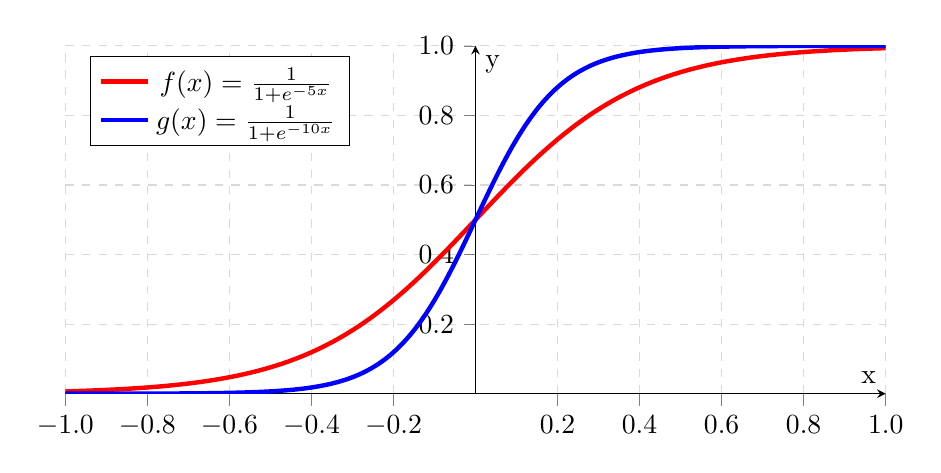
\begin{tikzpicture}
    \begin{axis}[
      legend pos=north west,
        axis x line=middle,
        axis y line=middle,
        x tick label style={/pgf/number format/fixed,
                            /pgf/number format/fixed zerofill,
                            /pgf/number format/precision=1},
        y tick label style={/pgf/number format/fixed,
                            /pgf/number format/fixed zerofill,
                            /pgf/number format/precision=1},
        grid = major,
        width=12cm,
        height=6cm,
        grid style={dashed, gray!30},
        xmin=-1,
        xmax= 1, 
        ymin= 0,  
        ymax= 1,   
        xlabel=x,
        ylabel=y,
        tick align=outside,
        enlargelimits=false]
      \addplot[domain=-1:1, red, ultra thick,samples=500] {1/(1+exp(-5*x))};
      \addplot[domain=-1:1, blue, ultra thick,samples=500] {1/(1+exp(-10*x))};
      \addlegendentry{$f(x)=\frac{1}{1+e^{-5x}}$}
      \addlegendentry{$g(x)=\frac{1}{1+e^{-10x}}$}
    \end{axis}
\end{tikzpicture}

\subsubsection{Decision Boundary}
Linear Decision Boundry:\\
$h_\theta(\vect{x}) = g(\theta_0 + \theta_1 x_1 + \theta_2 x_2)$\\
Predict ``y=1'' if $-3 + x_1 + x_2 \ge 0$\\

Non-linear Decision Boundry:\\
$h_\theta(\vect{x}) = g(\theta_0 + \theta_1 x_1 + \theta_2 x_2 + \theta_3 x_1^2 + \theta_4 x_2^2)$\\
Predict ``y=1'' if $-1 + x_1^2 + x_2^2 \ge 0$\\


\subsection{Logistic Regression Model}
\subsubsection{Cost Function}
Training set with m examples: $\{(x^{(1)}, y^{(1)}), (x^{(2)}, y^{(2)}), ...,  (x^{(m)}, y^{(m)})\}$\\

With n attributes, $\vect{x} = \begin{bmatrix}
x_0 \\ x_1 \\ x_2 \\ \vdots \\ x_n 
\end{bmatrix} \in \mathbb{R}^{n+1}$
$x_0 = 1, y \in \{0, 1\}$

$h_\theta(\vect{x}) = \frac{1}{1 + e^{-\vect{\theta}^T \vect{x}}}$ \\

\textbf{Logistic regression cost function} \\
$Cost(h_\theta(x), y)=\left\{
                \begin{array}{ll}
                  -log(h_\theta(x)), y = 1\\
                  -log(1 - h_\theta(x)), y = 0\\
                \end{array}
              \right.$

Cost = 0 if $y = 1$, $h_\theta(x) = 1$ \\
But as $h_\theta(x) \rightarrow 0, cost \rightarrow \infty $
Captures intuition that if $h_\theta(x) = 0$, but $y = 1$, we will penalize learning algorithm by a very large cost.\\

\newpage

\subsubsection{Simplified Cost Function and Gradient Descent}
\textbf{Logistic regression cost function} \\
$Cost(h_\theta(x), y)=\left\{
                \begin{array}{ll}
                  -log(h_\theta(x)), y = 1\\
                  -log(1 - h_\theta(x)), y = 0\\
                \end{array}
              \right.$\\

$J(\theta)= \frac{1}{m}\sum_{i=1}^{m} Cost(h_\theta(x^{(i)}), y^{(i)})$ \\

$ = -\frac{1}{m}[ \sum_{i=1}^{m} y^{(i)}log(h_\theta(x^{(i)})) + (1-y^{(i)})log(1 - h_\theta(x^{(i)}))]$\\

To fit parameters $\theta$: \\
\tab $\arg\min_{\theta} J(\theta)$ \\

To make a prediction given new $\vect{x}$:

\tab Output $h_\theta(\vect{x}) = \frac{1}{1 + e^{-\vect{\theta}^T \vect{x}}}$ \\

$\frac{\partial}{\partial \theta_j}(-log(h_\theta(x^{(i)}))) = (h_\theta(x^{(i)})-1)x^{(i)}$ \\
$\frac{\partial}{\partial \theta_j}(-log(1 - h_\theta(x))) = -h_\theta(x^{(i)})x^{(i)}$ \\

$\frac{\partial}{\partial \theta_j}[-y^{(i)}(log(h_\theta(x^{(i)})) - (1-y^{(i)})log(1 - h_\theta(x)))]$\\
$ = y^{(i)}(h_\theta(x^{(i)})-1)x^{(i)} + (1-y^{(i)})h_\theta(x^{(i)})x^{(i)} $\\
$ = (h_\theta(x^{(i)}) - y^{(i)}) x^{(i)}$\\

Algorithm looks identical to linear regression:\\
Repeat until convergence \{\\
\tab $\theta_j := \theta_j - \alpha \sum_{i=1}^{m}(h_\theta(x^{(i)} - y^{(i)})) x_{j}^{(i)}$ (simultaneously update all $\theta_j$) \\
\}\}\\

\subsubsection{Advanced Optimization}
Cost function $J(\theta)$. Want $\arg\min_\theta J(\theta)$\\
Given $\theta$, we have code that can compute $J(\theta)$ and $\frac{\partial}{\partial \theta_j}$ to perform gradient descent.\\

\textbf{Optimization algorithm}
\begin{itemize}
  \item Gradient descent
  \item Conjugate gradient
  \item BFGS
  \item L-BFGS
\end{itemize}

Advantages and disadvantages:
\begin{itemize}
  \item + No need to manually pick $\alpha$
  \item + Often faster than gradient descent
  \item - More complex
\end{itemize}

\subsection{Multiclass Classification}
\subsubsection{Multiclass Classification: One-vs-all}
Train a logistic regression classifier $h_\theta^{(i)}(x)$ for each class $i$ to predict the probability that $y = i$.\\

On a new input $x$ to make a prediction, pick the class $i$ that maximizes $h_\theta^{(i)}(x)$.

\newpage

\section{Regularization}
\subsection{Solving the Problem of Overfitting}
\subsubsection{The Problem of Overfitting}
Overfitting: If we have too many features, the learned hypothesis may fit the training set very well, but fail to generalize to new examples. \\

Options:
\begin{itemize}
  \item Reduce number of features
  \begin{itemize}
    \item Manually select which features to keep.
    \item Model selection algorithm
  \end{itemize}
  
  \item Regularization
  \begin{itemize}
    \item Keep all the features, but reduce magnitude/value of parameters $\theta_j$.
    \item Works well when we have a lot of features, each of which contribute a bit to predicting $y$.
  \end{itemize}
\end{itemize}

\subsubsection{Cost Function}
In regularized linear regression, we choose $\theta$ to minimize
$$J(\theta) = \frac{1}{2m}[ \sum_{i=1}^{m}(h_\theta(x^{(i)}) - y^{(i)})^2 + \lambda \sum_{i=1}^n \theta_{j}^2]$$

What if $\lambda$ is set to an extremely large value?
\begin{itemize}
  \item Algorithm works fine; setting $\lambda$ to be very large cannot hurt it
  \item Algorithm fails to eliminate overfitting
  \item Algorithm results in underfitting (Fails to fit even training set well)
  \item Gradient descent will fail to converge
\end{itemize}

\subsubsection{Regularized Linear Regression}
\textbf{Gradient descent}\\
Repeat until convergence \{\\
\tab $\theta_0 := \theta_0 - \alpha \frac{1}{m} \sum_{i=1}^{m}(h_\theta(x^{(i)} - y^{(i)})) x_{0}^{(i)}$ \\
\tab $\theta_j := \theta_j - \alpha [\frac{1}{m} \sum_{i=1}^{m}(h_\theta(x^{(i)} - y^{(i)})) x_{j}^{(i)} + \frac{\lambda}{m}\theta_j]$ (simultaneously update all $\theta_j$ except $\theta_0$) \\
\}\}\\

\textbf{Normal equation}\\\\
$\theta = (X^TX + \lambda \begin{bmatrix}
    0 & & & \\
    & 1 & & \\
    & & \ddots & \\
    & & & 1
  \end{bmatrix})^{-1} X^T y$

\subsubsection{Regularized Logistic Regression}
The same as section 1.1.3.

\newpage

\section{Neural Networks: Representation}
\subsection{Motivation}
\subsubsection{Non-linear Hypotheses}
\subsubsection{Neurons and the Brain}
Origins: Algorithms that try to mimic the brain. \\
Was very widely used in 80s and early 90s; Popularity diminished in late 90s. \\
Recent resurgence: State-of-art technique for many applications.

\subsection{Neural Networks}
\subsubsection{Model Representation}
Neuron model: Logistic unit. \\
Use Sigmoid (logistic) activation function. \\

$a_i^{(j)} = $ activation of unit i in layer j\\
$\theta^{(j)} = $ matrix of weights controlling function mapping from layer j to layer j+1.\\

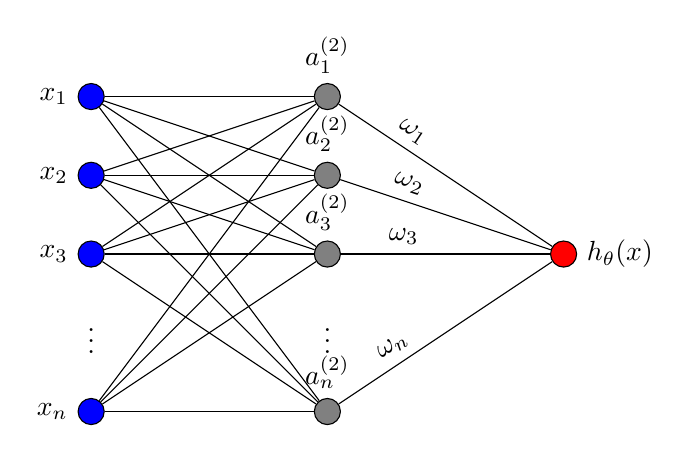
\begin{tikzpicture}
[   cnode/.style={draw=black,fill=#1,minimum width=3mm,circle},
]
    \node[cnode=red,label=0:$h_\theta(x)$] (s) at (6,-3) {};
    \node at (0,-4) {$\vdots$};
    \node at (3,-4) {$\vdots$};
    \foreach \x in {1,...,4}
    {   \pgfmathparse{\x<4 ? \x : "n"}
        \node[cnode=blue,label=180:$x_{\pgfmathresult}$] (x-\x) at (0,{-\x-div(\x,4)}) {};
        \node[cnode=gray,label=90:$a_{\pgfmathresult}^{(2)}$] (p-\x) at (3,{-\x-div(\x,4)}) {};
        \draw (p-\x) -- node[above,sloped,pos=0.3] {$\omega_{\pgfmathresult}$} (s);
    }
    \foreach \x in {1,...,4}
    {   \foreach \y in {1,...,4}
        {   \draw (x-\x) -- (p-\y);
        }
    }
\end{tikzpicture}\\

$a_1^{(2)} = g(\Theta^{(1)}_{10} x_0 + \Theta^{(1)}_{11} x_1 + \Theta^{(1)}_{12} x_2 + \Theta^{(1)}_{13} x_3)$ \\
$a_2^{(2)} = g(\Theta^{(1)}_{20} x_0 + \Theta^{(1)}_{21} x_1 + \Theta^{(1)}_{22} x_2 + \Theta^{(1)}_{23} x_3)$ \\
$a_3^{(2)} = g(\Theta^{(1)}_{30} x_0 + \Theta^{(1)}_{31} x_1 + \Theta^{(1)}_{32} x_2 + \Theta^{(1)}_{33} x_3)$ \\

$h_\Theta(x) = a_1^{(3)} = g(\Theta^{(2)}_{10} a_0^{(2)} + \Theta^{(2)}_{11} a_1^{(2)} + \Theta^{(2)}_{12} a_2^{(2)} + \Theta^{(2)}_{13} a_3^{(2)})$ \\

If network has $s_j$ units in layer $j$, $s_{j+1}$ units in layer $j+1$, then $\Theta^{(j)}$ will be of dimension $s_{j+1}$ by $s_{j} + 1$. \\

$\vect{x} = 
\begin{bmatrix}
x_0 \\ x_1 \\ x_2 \\ \vdots \\ x_n 
\end{bmatrix}
\tab
\vect{z}^{(2)} = 
\begin{bmatrix}
\vect{z}^{(2)}_1 \\ \vect{z}^{(2)}_2 \\ \vect{z}^{(2)}_3 \\ \vdots \\ \vect{z}^{(2)}_n 
\end{bmatrix} \\\\$

$z^{(2)} = \Theta^{(1)}x = \Theta^{(1)} a^{(1)}$\\
$a^{(2)} = g(z^{(2)})$\\

Add $a_0^{(2)} = 1$.\\

$z^{(3)} = \Theta^{(2)}a^{(2)}$\\
$h_\theta(x) = a^{(3)} = g(z^{(3)})$

\section{Neural Networks: Learning}
\subsection{Cost Function and Backpropagation}
\subsubsection{Cost Function}
\textbf{Binary classification}\\
y = 0, y = 1. (1 output unit). \\

\textbf{Multi-class classification with K classes}\\

E.g.$\begin{bmatrix}
1 \\ 0 \\ 0 \\ 0
\end{bmatrix},
\begin{bmatrix}
0 \\ 1 \\ 0 \\ 0
\end{bmatrix},
\begin{bmatrix}
0 \\ 0 \\ 1 \\ 0
\end{bmatrix},
\begin{bmatrix}
0 \\ 0 \\ 0 \\ 1
\end{bmatrix}$\\\\

$y \in \mathbb{R}^{n+1}, K$ output units.\\

\textbf{Cost function}\\

Logistic regression:\\
$$J(\theta) = -\frac{1}{m}[\sum_{i=1}^{m}y^{(i)}log(h_\theta(x^{(i)})) + (1-y^{(i)})log(1-h_\theta(x^{(i)}))] + \frac{\lambda}{2m} \sum_{j=1}^n \theta_{j}^2$$

Neural network:\\
$h_\theta(x) \in \mathbb{R}^{K}$, $(h_\theta(x))_i$ = $i^{th}$ output.\\
$$J(\Theta) = -\frac{1}{m}[\sum_{i=1}^{m}\sum_{k=1}^{K}y_k^{(i)}log(h_\theta(x^{(i)})_k) + (1-y^{(i)}_k)log(1-h_\theta(x^{(i)})_k)] + \frac{\lambda}{2m} \sum_{l=1}^{L-1}\sum_{i=1}^{s_l}\sum_{j=1}^{s_{l+1}} (\theta_{ji}^{(l)})^2$$


\subsubsection{Backpropagation Algorithm}
\textbf{Given one training example $(x, y)$}\\

Forward propagation: \\
$a^{(1)} = x$\\
$z^{(2)} = \Theta^{(1)}a^{(1)}$\\
$a^{(2)} = g(z^{(2)})$ (add $a_0^{2}$)\\
$z^{(3)} = \Theta^{(2)}a^{(2)}$\\
$a^{(3)} = g(z^{(3)})$ (add $a_0^{3}$)\\
$z^{(4)} = \Theta^{(3)}a^{(3)}$\\
$a^{(4)} = h_\Theta(x) = g(z^{(4)})$\\

Gradient computation: Backpropagation algorithm: \\
Intuition: $\delta_j^{(l)}$ = ``error'' of node j in layer $l$.\\

For each output unit (layer L = 4) \\
$\delta^{(4)} = a^{(4)} - y$ \\
$\delta^{(3)} = (\Theta^{(3)})^T \delta^{(4)} .* g'(z^{(3)})$ \tab $g'(z) = a .* (1-a)$ \\
$\delta^{(2)} = (\Theta^{(2)})^T \delta^{(3)} .* g'(z^{(2)})$ \\

$\frac{\partial}{\partial \Theta_{ij}^{(l)}}J(\Theta) = a_j^{(l)} \delta_i^{(l+1)}$ (ignore $\lambda$ or $\lambda = 0$)\\

\newpage

\textbf{Backpropagation algorithm}\\
Training set $\{(x^{(1)}, y^{(1)}),(x^{(2)}, y^{(2)}),...,(x^{(m)}, y^{(m)})\}$ \\
Set $\Delta_{ij}^{(l)} = 0$ for all $l, i, j$ \\
For $i = 1$ to $m$ \\
\tab Set $a^{(1)} = x^{(i)}$ \\
\tab Perform forward propagation to compute $a^{(l)}$ for $l = 2, 3, ..., L$ \\
\tab Using $y^{(i)}$, compute $\delta^{(L)} = a^{(L)} - y^{(i)}$ \\
\tab Compute $\delta^{(L-1)}, \delta^{(L-2)}, ..., \delta^{(2)}$ \\
\tab $\Delta_{ij}^{(l)} := \Delta_{ij}^{(l)} + a_j^{(l)} \delta_i^{(l+1)}$ \\

$D_{ij}^{(l)} := \frac{1}{m} \Delta_{ij}^{(l)} + \lambda \theta_{ij}^{(l)}$, if $j \ne 0$ \\
$D_{ij}^{(l)} := \frac{1}{m} \Delta_{ij}^{(l)}$, \tab if $j = 0$ \\

$\frac{\partial}{\partial \Theta_{ij}^{(l)}}J(\Theta) = D_{ij}^{(l)}$

\subsection{Backpropagation in Practice}
\subsubsection{Implementation Note: Unrolling Parameters}
Skip
\subsubsection{Gradient Checking}
\textbf{Implementation Note}
\begin{itemize}
  \item Implement backprop to compute \textbf{DVec} 
  \item Implement numerical gradient check to compute \textbf{gradApprox}
  \item Make sure they give similar values
  \item Turn off gradient checking. Using backprop code for learning.
\end{itemize}

\textbf{Important}
Be sure to disable your gradient checking code before training your classifier. If you run numerical gradient computation on every iteration of gradient descent, your code will be very slow.

\subsubsection{Random Initialization}
For gradient descent and advanced optimization method, need initial value for $\Theta$.\\

Initialize each $\Theta_{ij}^{(l)}$ to a random value in $[-\epsilon, \epsilon].$

\subsubsection{Putting It Together}
\textbf{Training a neural network}
Pick a network architecture (connectivity pattern between neurons) \\
No. of input units: Dimension of features $x^{(i)}$ \\
No. output units: Number of classes \\
Reasonable default: 1 hidden layer, or if $> 1$ hidden layer, have same no. of hidden units in every layer (usually the more the better) \\  

Steps:\\
1. Randomly initialize weights.\\
2. Implement forward propagation to get $h_\Theta(x^{(i)})$ for any $x^i$\\
3. Implement code to compute cost function $J(\Theta)$ \\
4. Implement backprop to compute partial derivates $\frac{\partial}{\partial \theta_{jk}^{(l)}} J(\Theta)$ \\
5. Use gradient checking to compare $\theta_{jk}^{(l)} J(\Theta)$ computed using backpropagation vs. numerical estimate of gradient of $J(\Theta)$. Then disable gradient checking code.\\
6. Use gradient descent or advanced optimization method with backpropagation to try to minimize $J(\Theta)$ as a function of parameters $\Theta$.

\newpage

\section{Advice for Applying Machine Learning}
\subsection{Evaluating a Learning Algorithm}
\subsubsection{Deciding What to Try Next}
Machine learning diagnostic:A test that you can run to gain insight what is / is not working with a learning algorithm and gain guidance as to how to improve its performance.\\

Diagnostics can take time to implement, but doing so can be a very good use of your time.
\subsubsection{Evaluating a Hypothesis}
Learn parameter $\theta$ from training data. \\
Compute test set error. \\
Misclassification error.
\subsubsection{Model Selection and Train / Validation / Test Sets}
Divide data set into training set, cross validation set and test set.

\subsection{Bias vs. Variance}
\subsubsection{Diagnosing Bias vs. Variance}


\subsubsection{Regularization and Bias / Variance}
\subsubsection{Learning Curves}
\subsubsection{Deciding What to do Next Revisited}

\section{Machine Learning System Design}
\subsection{Building a Spam CLassifier}
\subsubsection{Prioritizing What to Work On}
\subsubsection{Error Analysis}
\textbf{Recommended Approach}\\
1. Start with a simple algorithm that you can implement quickly. Implement it and test it on your cross-validation data. \\
2. Plot learning curves to decide if more data, more features, etc. Are likely to help. \\
3. Error analysis: Manually examine the exmaples (in cross validation set) that your algorithm made errors on. See if you spot any systematic trend in that type of exmaples it is making errors on. \\

Error analysis may not be helpful for deciding if this is likely to improve performance. Only solution is to try it and see if it works.

\subsection{Handling Skewed Data}
\subsubsection{Error Metrics for Skewed Classes}
\begin{center}
\textbf{Comparison} \\
\begin{tabular}{ | c | c | c | }
\hline
 & Predicted as positive & Predicted as negative \\ 
\hline
Actually positive & True Positive (TP) & False Negative (FN) \\  
\hline
Actually negative & False Positive (FP) & True Negative (TN) \\
\hline
\end{tabular}
\end{center}

\begin{center}
Precision = $\frac{TP}{TP + FP}$ \tab Recall = $\frac{TP}{TP + FN}$ \\
\end{center}

\subsubsection{Trading Off Precision and Recall}
Suppose we want to predict $y = 1$ (cancer) only if very confident, there will be high precision and low recall. \\
Suppose we want to avoid missing too many causes of cancer (avoid false negatives), there will be high recall and low precision. \\
To compare precision and recall, use $F_1$ score: $2\frac{PR}{P+R}$

\subsection{Using Large Data Sets}
\subsubsection{Data For Machine Learning}
\textbf{Large data rationale}\\

Assume features have sufficient information to predict $y$ accurately. A useful test is by asking the question that given the input $x$, can a human expert confidently predict $y$.\\

For large data, use a learning algorithm with many parameters (e.g. logistic regression/linear regression with many features; neural network with many hidden units). \\

Use a very lage training set to prevent overfit.\\

\end{document}